\documentclass[10pt,a4paper]{article}
\usepackage[margin=2cm]{geometry}
\usepackage{booktabs}
\usepackage{graphicx}
\usepackage{amsmath}
\usepackage{enumitem}
\usepackage{caption}
\usepackage{tabularx}
\usepackage{float}
\setlist{nosep,leftmargin=*}
\setlength{\parindent}{0pt}
\setlength{\parskip}{4pt}
\captionsetup{font=small,skip=3pt}

\title{\vspace{-1.5cm}CS6886 Assignment 5: Optimising Attention on a CPU}
\author{Shaik Sadik \quad (CS26S010)}
\date{}

\begin{document}
\maketitle
\vspace{-1.2cm}

\paragraph{Setup.} Apple M1 MacBook Air, macOS 15.1.1, Homebrew clang 23.1.5 with \texttt{-O3 -march=native} (\texttt{-fopenmp} for omp). Times are the driver's median of 5 runs. All tables come from one session (\texttt{results.csv}). Every variant passes \texttt{make check} on every input (max error $4.7\times10^{-6}$).

%--------------------------------------------------------------------------
\section*{Q1. Machine}

\noindent\begin{tabularx}{\linewidth}{@{}lX@{}}
\toprule
CPU & Apple M1 (Firestorm P-cores + Icestorm E-cores), ARMv8.5-A \\
Cores & 8 physical, 8 logical (no SMT); 4 P + 4 E \\
Clock & P-core max 3.204 GHz, E-core max 2.064 GHz \\
SIMD / FMA & NEON 128-bit (4 FP32 lanes); 4 FMA units per P-core, 2 per E-core; 32 vector registers \\
Caches & L1D 128 KB (P) / 64 KB (E); L2 12 MB shared by P-cores, 4 MB shared by E-cores; 8 MB SLC; 128 B lines \\
Memory & 8 GB LPDDR4X-4266, 128-bit bus \\
\bottomrule
\end{tabularx}
{\small Cores, caches, RAM size and clock steps from \texttt{sysctl}, \texttt{system\_profiler} and \texttt{powermetrics}. SIMD width, FMA units, SLC and memory speed and bus width from public M1 documentation (not exposed by macOS).}

\textbf{Peak FP32.} One FMA on 4 lanes = 8 FLOP.
\begin{align*}
\text{1 P-core} &= 4 \text{ lanes} \times 2 \times 4 \text{ FMA units} \times 3.204\text{ GHz} = \mathbf{102.5\ GFLOP/s}\\
\text{1 E-core} &= 4 \times 2 \times 2 \times 2.064\text{ GHz} = 33.0\text{ GFLOP/s}\\
\text{All cores} &= 4 \times 102.53 + 4 \times 33.02 = \mathbf{542.2\ GFLOP/s}
\end{align*}
\textbf{Bandwidth} $= 16\text{ B} \times 4.266\text{ GT/s} = \mathbf{68.3\ GB/s}$.\quad
\textbf{Ridge point} $=$ peak / bandwidth: one core $102.5/68.3 = \mathbf{1.50}$ FLOP/B, all cores $542.2/68.3 = \mathbf{7.94}$ FLOP/B.

%--------------------------------------------------------------------------
\section*{Q2. Naive baseline}

\begin{tabular}{@{}rrrrr@{}}
\toprule
N & d & time (ms) & GFLOP/s & \% of 1-core peak \\
\midrule
1024 & 64 & 105.1 & 2.55 & 2.5 \\
2048 & 64 & 421.0 & 2.55 & 2.5 \\
4096 & 64 & 1720.2 & 2.50 & 2.4 \\
4096 & 128 & 3653.3 & 2.35 & 2.3 \\
\bottomrule
\end{tabular}

\textbf{Scaling.} Doubling N multiplies the time by 4.0--4.1 and doubling d by 2.1, so time $\propto N^2 d$, the same as the FLOP count ($4N^2d$). GFLOP/s stays constant, so the cost per FLOP does not depend on problem size.

\textbf{Where the time goes.} Timing each phase separately (N=4096, d=64): $QK^\top$ 19\% (6.5 GFLOP/s), softmax 3\%, $SV$ 78\% (1.6 GFLOP/s).
\begin{itemize}
\item Each dot product adds into one variable. C does not allow the compiler to reorder floating-point additions, so the assembly contains a chain of dependent adds (\texttt{fadd s1, s1, \ldots}). Each add waits for the previous one, so the core is limited by add latency, not by its FMA throughput.
\item Compiling with \texttt{-ffast-math} (which allows reordering) made $QK^\top$ 3.9$\times$ faster but did not change $SV$. In $SV$ the inner loop walks down a column of $V$ (stride $d$), so it runs as scalar code (the compiler's vector version is only used when the stride is 1). This is one scalar FMA chain: with a 4-cycle FMA latency, $2 \times 3.2/4 = 1.6$ GFLOP/s.
\end{itemize}

%--------------------------------------------------------------------------
\section*{Q3. Optimisations}

\begin{table}[H]
\centering\footnotesize\setlength{\tabcolsep}{3.5pt}
\begin{tabular}{@{}l rrrr rrrr@{}}
\toprule
& \multicolumn{4}{c}{time (ms)} & \multicolumn{4}{c}{GFLOP/s \;(\% of 1-core peak) \;[speedup over naive]} \\
\cmidrule(lr){2-5}\cmidrule(l){6-9}
N, d & 1024, 64 & 2048, 64 & 4096, 64 & 4096, 128 & 1024, 64 & 2048, 64 & 4096, 64 & 4096, 128 \\
\midrule
naive & 105.1 & 421.0 & 1720.2 & 3653.3 & 2.6 (2\%) [1.0] & 2.6 (2\%) [1.0] & 2.5 (2\%) [1.0] & 2.4 (2\%) [1.0] \\
loops & 14.6 & 57.0 & 226.5 & 376.0 & 18.4 (18\%) [7.2] & 18.8 (18\%) [7.4] & 19.0 (18\%) [7.6] & 22.9 (22\%) [9.7] \\
tiled & 6.1 & 20.1 & 84.8 & 130.4 & 44.1 (43\%) [17.2] & 53.5 (52\%) [21.0] & 50.6 (49\%) [20.3] & 65.9 (64\%) [28.0] \\
fused & 4.9 & 19.3 & 77.2 & 122.9 & 55.3 (54\%) [21.6] & 55.6 (54\%) [21.8] & 55.6 (54\%) [22.3] & 69.9 (68\%) [29.7] \\
best & 4.3 & 14.0 & 55.7 & 100.2 & 63.1 (62\%) [24.7] & 76.6 (75\%) [30.1] & 77.1 (75\%) [30.9] & 85.7 (84\%) [36.5] \\
\bottomrule
\end{tabular}
\caption{Single-threaded results.}
\end{table}

\begin{figure}[H]
\centering
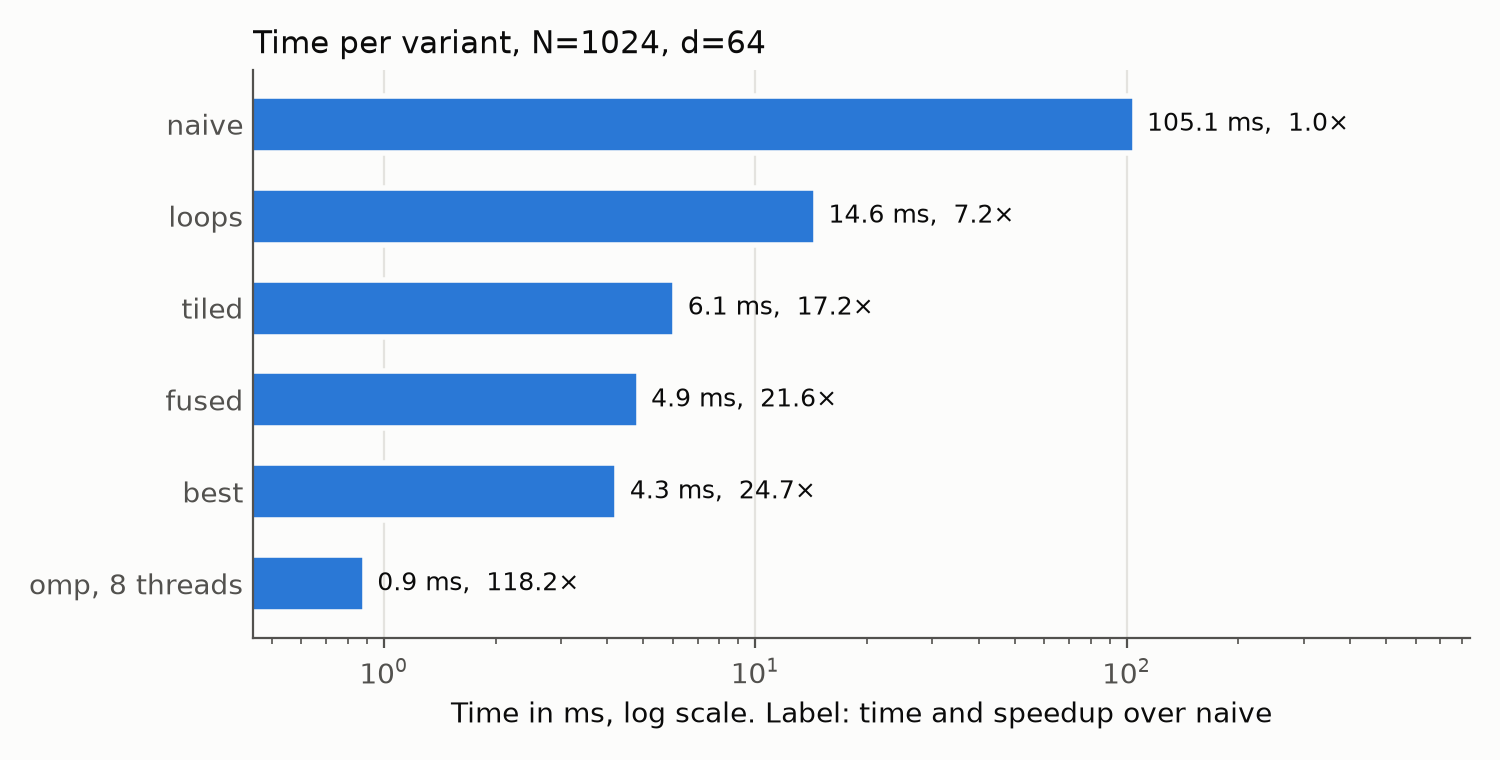
\includegraphics[width=0.49\linewidth]{../plots/time_N1024_d64.png}\hfill
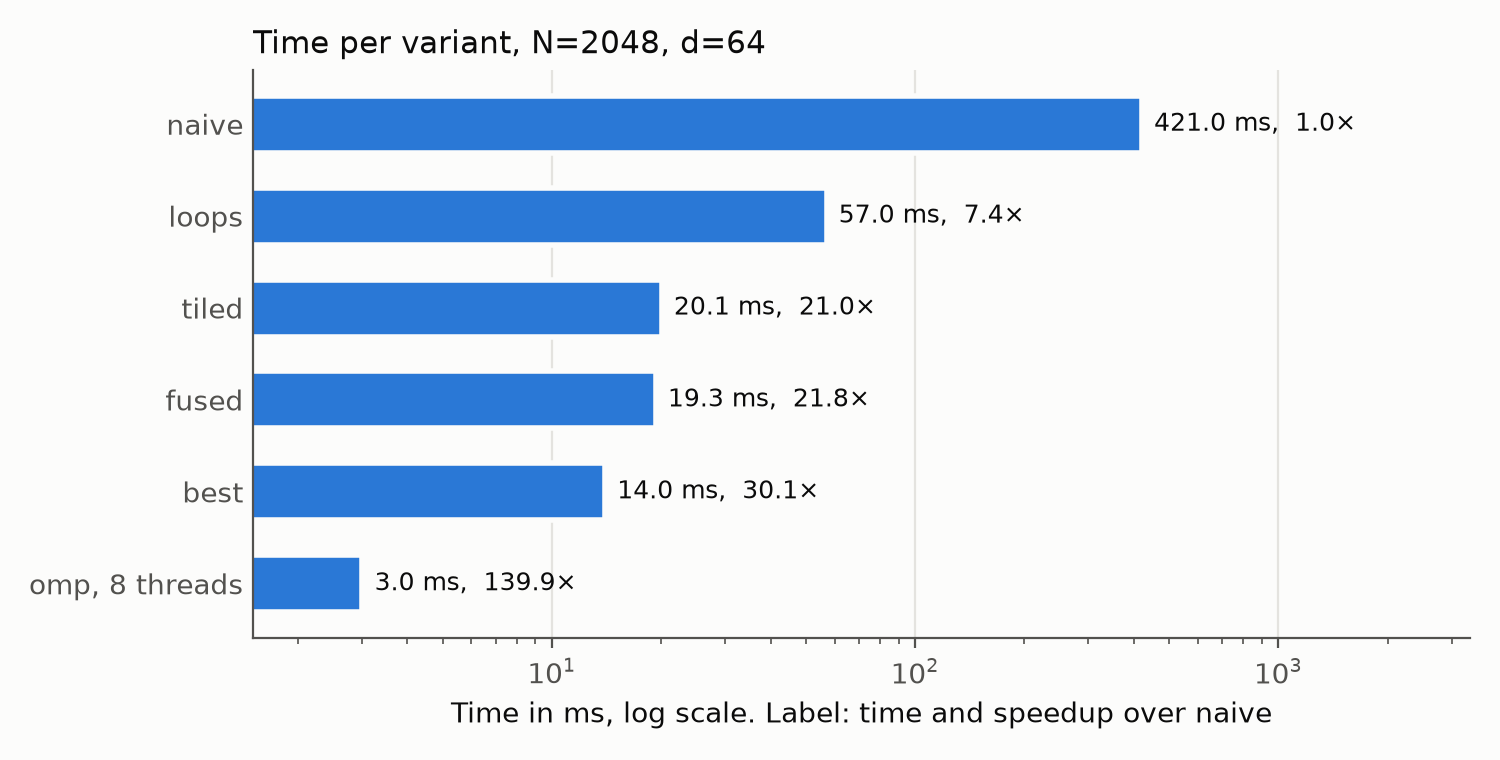
\includegraphics[width=0.49\linewidth]{../plots/time_N2048_d64.png}\\[2pt]
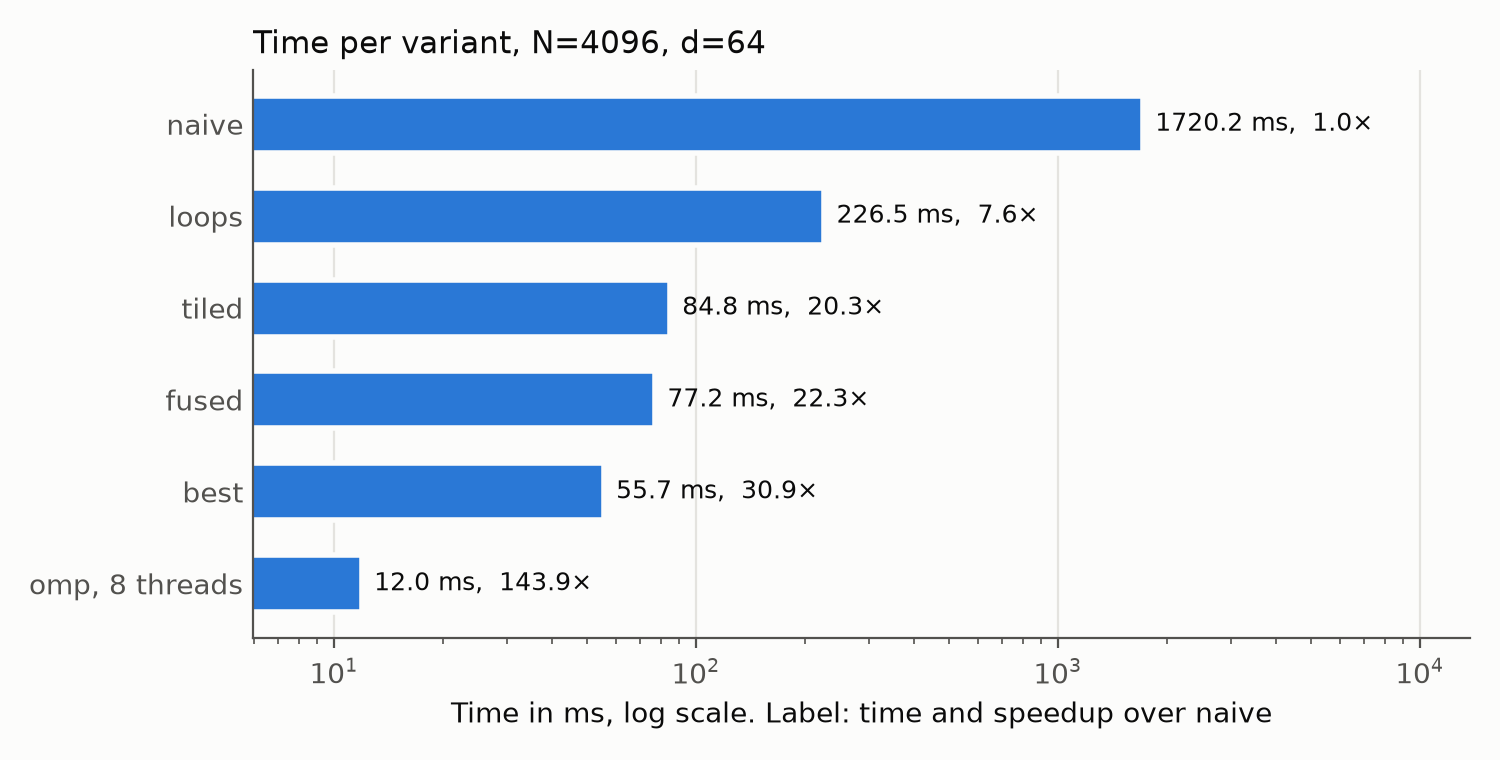
\includegraphics[width=0.49\linewidth]{../plots/time_N4096_d64.png}\hfill
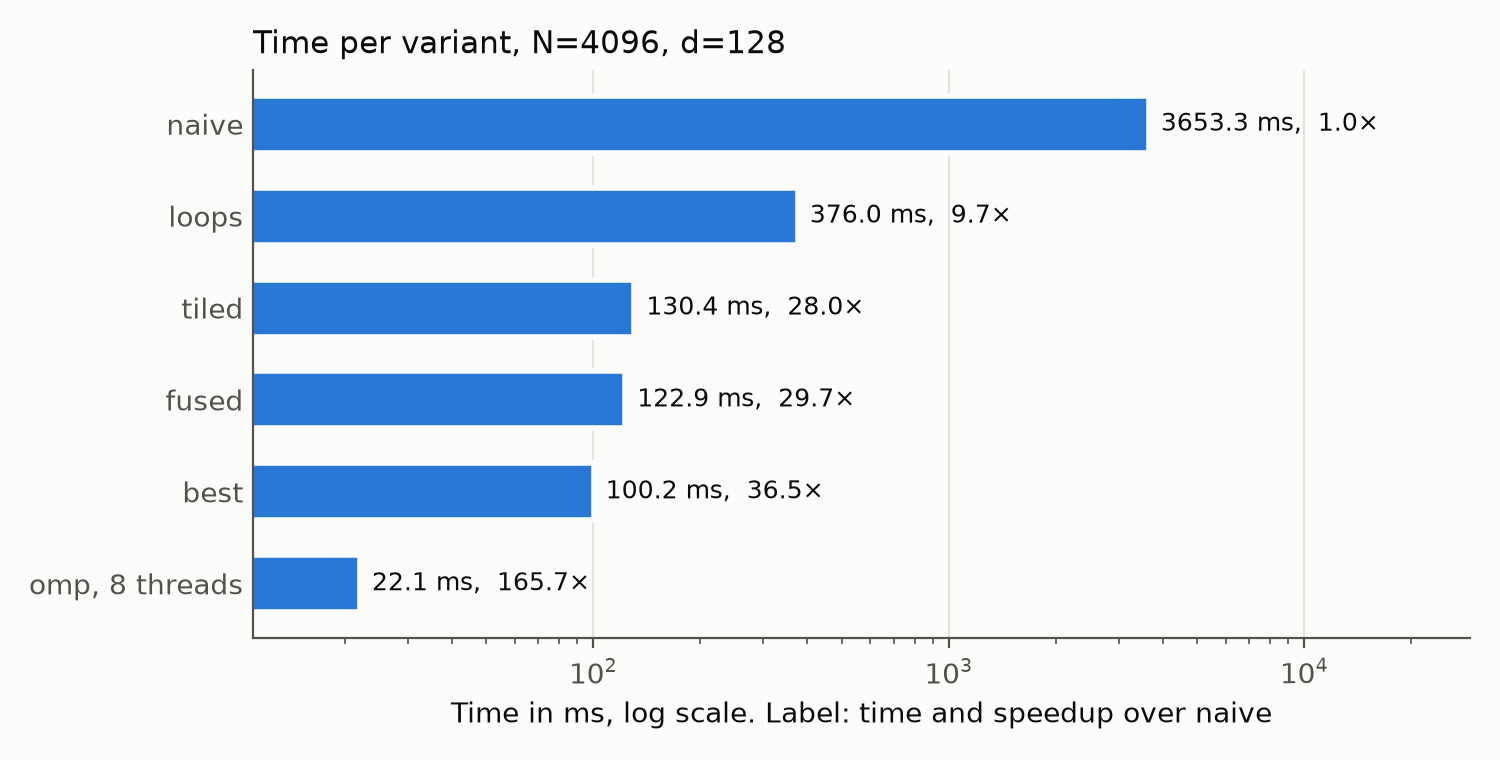
\includegraphics[width=0.49\linewidth]{../plots/time_N4096_d128.png}
\caption{Time of every variant on each input (log scale; label: time and speedup over naive; omp at 8 threads).}
\end{figure}

\textbf{(a) loops.} Reordered both products so the innermost loop runs over contiguous memory and writes a different element each iteration: $QK^\top$ uses order $i$-$k$-$j$ over a transposed copy of $K$, and $SV$ uses $i$-$j$-$k$ (\texttt{O[i][k] += S[i][j]*V[j][k]}), which reads rows of $V$ instead of columns. There is no reduction into one variable, so the compiler vectorises both loops without \texttt{-ffast-math}.
\emph{Limit afterwards:} the accumulators are rows of $S$ or $O$ in memory, so every vector FMA needs 2 loads and 1 store. Both products run at about 21--24 GFLOP/s, limited by load/store throughput while the FMA units are mostly idle. Softmax grows to 14\% of the time.

\textbf{(b) tiled.} Register tiling: each kernel call computes a $4\times16$ output block held in 16 NEON registers for the whole reduction, and stores it once. Each step does about 5 loads per 16 FMAs and no stores. 16 independent accumulators are enough to hide the FMA latency (4 units $\times$ 4 cycles). Cache tiling: $K$ is packed into 16-row panels and processed in blocks of 64 KB that stay in L1.
The products became 3--4$\times$ faster (about 75 GFLOP/s). Removing the cache blocking made no difference (2--4\% faster), so the gain comes from register tiling.
\emph{Limit afterwards:} softmax (scalar \texttt{expf}) did not change and is now 40\% of the time at d=64. The $N\times N$ matrix $S$ (64 MB) is still written to and read from DRAM.

\textbf{(c) fused.} Rows are processed in blocks of 4: compute the $4\times N$ scores, apply softmax, and multiply by $V$ immediately. The scores live in a 64 KB buffer that stays in L1, so the $N\times N$ matrix is never stored (64 MB $\rightarrow$ 64 KB). The kernels are the same as in tiled. They run at about 90 GFLOP/s. Fused is 6--10\% faster than tiled at N=4096 and 4\% at N=2048. N=1024 runs last only about 5 ms and vary by up to 30\% between sessions, so they are not compared.
\emph{Limit afterwards:} softmax is 41\% of the time.

\textbf{(d) best.} Fused plus a vectorised exponential. $e^x = 2^n e^r$ with $n=\text{round}(x/\ln2)$, $r = x - n\ln2$. $e^r$ is a degree-7 polynomial and $2^n$ is written directly into the float's exponent bits. This computes 4 values per instruction with no library call. It is 4.2$\times$ faster per element than \texttt{expf} with max relative error $1.2\times10^{-7}$.
\emph{Why it works:} at N=4096 there are $N^2 = 16.8$M exponentials, each now 1.26 ns cheaper, which predicts a 21.2 ms saving. The measured saving is 21.1 ms (d=64) and 21.9 ms (d=128).
\emph{Limit afterwards:} the matrix products are at about 90\% of peak. The rest of softmax (the vector exp and the max and normalise passes) is estimated at about 23\% of the time.

%--------------------------------------------------------------------------
\section*{Q4. OpenMP}

\texttt{attn\_omp.c} is best with \texttt{\#pragma omp parallel for} over the 4-row blocks. Each block writes only its own rows of $O$, so no locks are needed. Each thread has its own score buffer. Blocks are handed out dynamically.

\begin{table}[H]
\centering\footnotesize\setlength{\tabcolsep}{4pt}
\begin{tabular}{@{}r rrr rrr rrr rrr@{}}
\toprule
& \multicolumn{3}{c}{N=1024, d=64} & \multicolumn{3}{c}{N=2048, d=64} & \multicolumn{3}{c}{N=4096, d=64} & \multicolumn{3}{c}{N=4096, d=128} \\
\cmidrule(lr){2-4}\cmidrule(lr){5-7}\cmidrule(lr){8-10}\cmidrule(l){11-13}
threads & ms & speedup & eff. & ms & speedup & eff. & ms & speedup & eff. & ms & speedup & eff. \\
\midrule
1 & 3.54 & 1.00 & 100\% & 14.01 & 1.00 & 100\% & 55.46 & 1.00 & 100\% & 99.86 & 1.00 & 100\% \\
2 & 2.19 & 1.62 & 81\% & 8.31 & 1.69 & 84\% & 29.37 & 1.89 & 94\% & 51.90 & 1.92 & 96\% \\
4 & 1.04 & 3.39 & 85\% & 4.22 & 3.32 & 83\% & 15.91 & 3.49 & 87\% & 28.43 & 3.51 & 88\% \\
6 & 0.89 & 3.97 & 66\% & 3.36 & 4.17 & 69\% & 13.49 & 4.11 & 69\% & 24.35 & 4.10 & 68\% \\
8 & 0.89 & 3.98 & 50\% & 3.01 & 4.65 & 58\% & 11.95 & 4.64 & 58\% & 22.05 & 4.53 & 57\% \\
\bottomrule
\end{tabular}
\caption{omp time, speedup and parallel efficiency (speedup / threads), relative to omp with 1 thread. Best: 11.95 ms at N=4096, d=64 (359 GFLOP/s, 144$\times$ faster than naive).}
\end{table}

\textbf{Scaling.}
\begin{itemize}
\item \textbf{1--4 threads} run on the 4 P-cores and scale almost linearly. Efficiency drops to 87\% at 4 threads mainly because the P-core clock falls as more cores are busy (measured with \texttt{powermetrics}: 3.14 GHz with 1 thread, 2.84 GHz with 4, 2.55 GHz with 8). $2.84/3.14 = 90\%$ is already the upper limit at 4 threads.
\item \textbf{5--8 threads} add the E-cores, which have half the FMA units and a lower clock (peak 33.0 vs 102.5 GFLOP/s, about $1/3$ of a P-core), while the P-cores slow down further. So 4 extra cores add only about 33\% (4 $\rightarrow$ 8 threads: 15.91 $\rightarrow$ 11.95 ms).
\item \textbf{Scheduling matters} because the cores are unequal. With a static schedule each thread gets the same amount of work, so the P-cores wait for the E-cores: going from 4 to 5 threads made it slower (17.1 $\rightarrow$ 17.6 ms) and 8 threads reached only 14.4 ms. A dynamic schedule lets faster cores take more blocks (12.5 ms at 8 threads in the same test).
\end{itemize}

%--------------------------------------------------------------------------
\section*{Q5. Roofline}

\begin{figure}[H]
\centering
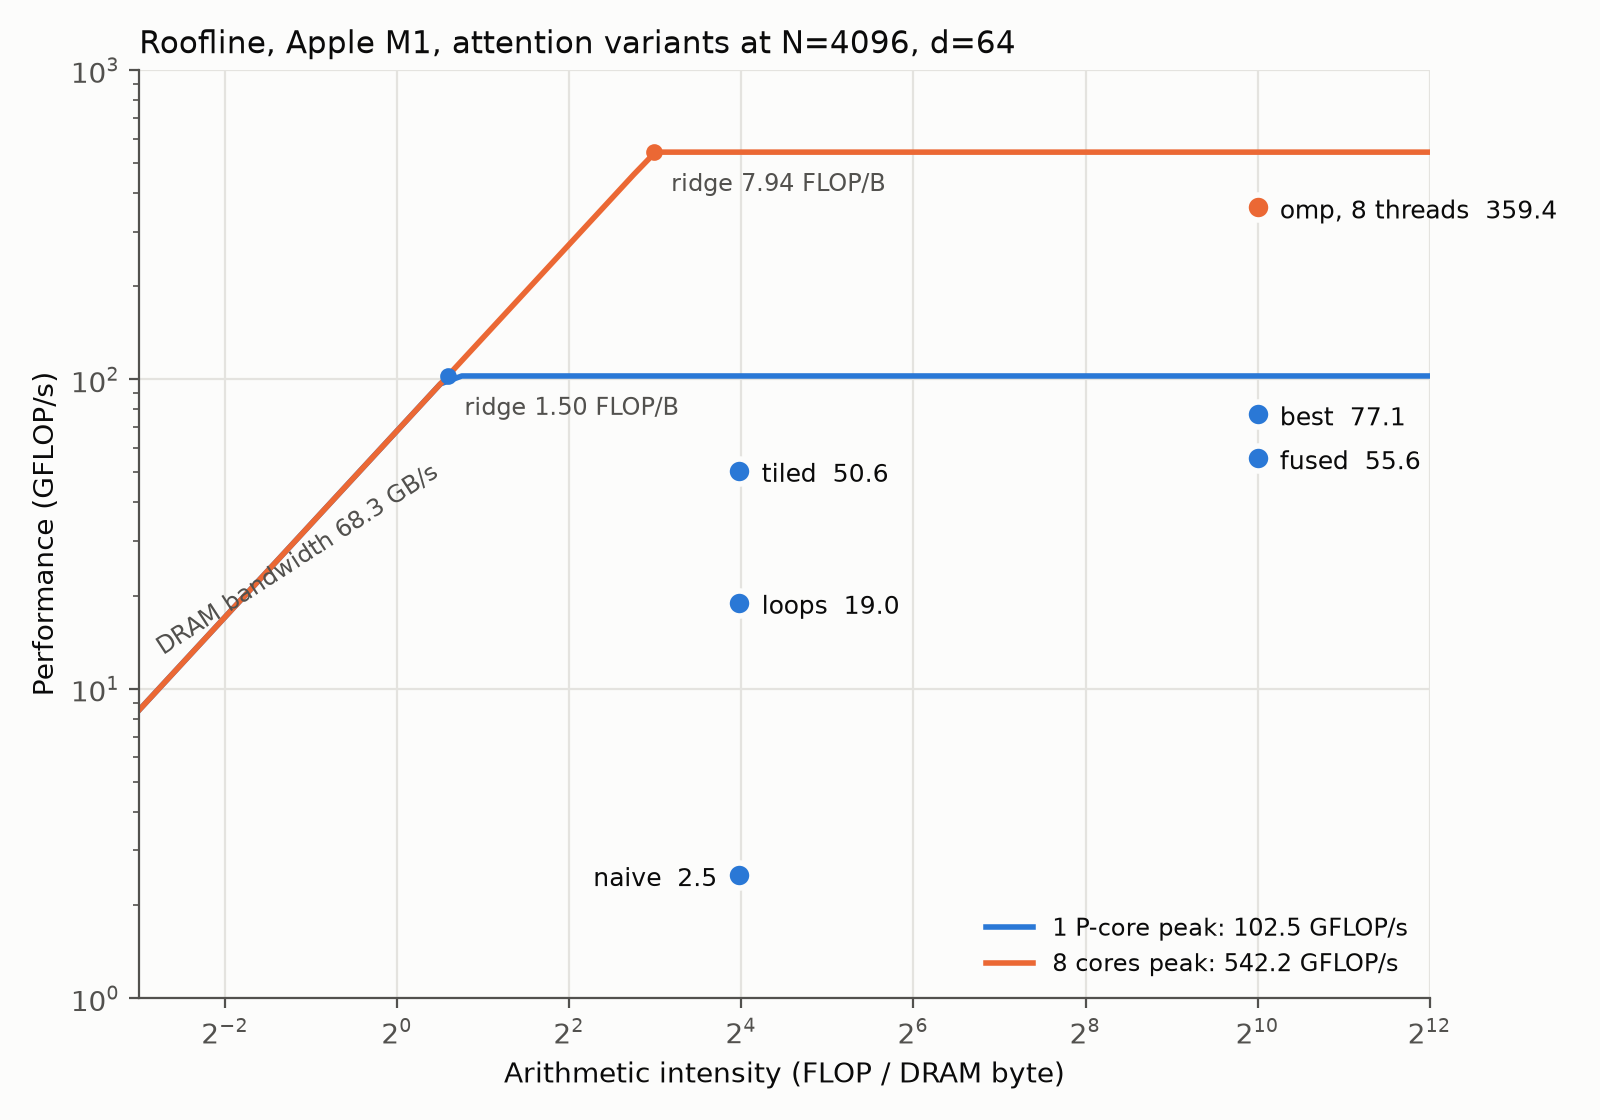
\includegraphics[width=0.72\linewidth]{../plots/roofline.png}
\caption{Roofline from the Q1 numbers (68.3 GB/s; 102.5 and 542.2 GFLOP/s) with every variant at N=4096, d=64.}
\end{figure}

\textbf{Arithmetic intensity} $=$ FLOPs / DRAM bytes. FLOPs $= 4N^2d$ for all variants. Bytes:
\begin{itemize}
\item \textbf{naive, loops, tiled} store $S$ ($N^2$ floats, 64 MB, larger than all caches). $S$ crosses DRAM 4 times (written by $QK^\top$, read and written by softmax, read by $SV$), plus reading $Q,K,V$ and writing $O$ once: $16N^2 + 16Nd$ bytes. AI $= \frac{4N^2d}{16N^2+16Nd} \approx d/4 = \mathbf{15.75}$.
\item \textbf{fused, best, omp} never store $S$, so only $Q,K,V,O$ cross DRAM: $16Nd$ bytes. AI $= \frac{4N^2d}{16Nd} = N/4 = \mathbf{1024}$.
\end{itemize}

\textbf{What limits each variant.} Every variant has AI $\ge 15.75$, to the right of both ridge points (1.50 and 7.94), so none is limited by memory bandwidth. The distance below the roof is caused by how well each variant uses the core:

\begin{tabular}{@{}lrrl@{}}
\toprule
variant & AI & GFLOP/s & limit \\
\midrule
naive & 15.75 & 2.5 & serial add chains (add latency) \\
loops & 15.75 & 19.0 & loads/stores: 2 loads + 1 store per FMA \\
tiled & 15.75 & 50.6 & softmax with scalar \texttt{expf} (40\%); $S$ stored in DRAM \\
fused & 1024 & 55.6 & softmax with scalar \texttt{expf} (41\%) \\
best & 1024 & 77.1 & remaining softmax passes; products at $\approx$90\% of peak \\
omp (8 threads) & 1024 & 359.4 & lower clocks with all cores busy; slower E-cores \\
\bottomrule
\end{tabular}

Naive, loops and tiled have the same AI but differ by 20$\times$ in speed: those gains came from better use of the core, not from less memory traffic. Fusion moved the variants to a much higher AI, but since they were already compute-bound, it gave only a small speedup.

\end{document}
